\chapter{System design}\label{ch:system_design}

In the previous chapter, we have extracted the functional and non-functional requirements of our system. Subsequently, we broke down our system into use cases in the use case model. Furthermore, we have described the entities of our system and the relationships between them using an Analysis Object Models and we presented 3 activity diagrams that depict the workflows in our system.

In this chapter we map our analysis into the solution domain. We first identify our design goals in section \ref{sec:design_goals}. In section \ref{sec:subsystem_decomposition}, we group the objects that we have identified in the analysis object models into subsystems, and we discuss the dependencies between those subsystems. In section \ref{sec:hardware_software_mapping} we present the hardware and software components used to implement our system. Lastly, section \ref{sec:persistent_data_management} presents the structure of our system's persistent data.


\section{Design Goals}\label{sec:design_goals}

In the previous chapter we have defined our non-functional requirements. In this section, we use those non-functional requirements to extract our design goals, and we use those design goals as a compass for our system design. Defining our design goals allows us to make consistent design decisions across our different subsystems. Table \ref{tab:DG} lists our non-functional requirements and their corresponding design goal. There are 5 types of possible design criteria from which the design goals can be selected: performance, dependability, cost, maintenance and end user criteria \cite{bruegge2004object}.

\begin{table}
  \centering
  \begin{tabular}{ | l | p{5cm} | l | }
    \hline
    \textbf{Requirement} & \textbf{Design Goal} & \textbf{Criteria} \\ \hline
    \textbf{Adaptability} & The system should create a convolutional neural network that can accommodate the addition of new classes. & Performance \\ \hline
    \textbf{Accuracy} & The system should utilize real and synthetic images to train a CNN model to classify different small parts with high accuracy. & Performance \\ \hline
  \end{tabular}
  \caption{Non-functional requirements and their corresponding design goals.}
  \label{tab:DG}
\end{table}


\section{Subsystem Decomposition}\label{sec:subsystem_decomposition}

Figure \ref{fig:SSD} depicts our system's subsystem decomposition. Our system is divided into 3 subsystems. \textbf{SyntheticImageSubsystem} is responsible for providing our system with synthetic images. It consists of 4 main components: \textbf{3DScanner}, \textbf{3DScanningSoftware}, \textbf{3DScanningSoftware}, \textbf{SyntheticScene} and \textbf{3DModelingSoftware}. The 3DScanner scans \textbf{SmallParts} and outputs raw 3D model, which are processes by the 3DModelingSoftware to create a \textbf{3DModel}. The SyntheticScene generates an artificial environment. The 3DModelingSoftware places the 3D models in the environment created by SyntheticScene, and renders \textbf{SyntheticImages} of the 3D models.

On the other hand, \textbf{RealImageSubsystem} is responsible for providing our system with real images. The \textbf{Camera} is used to take real images of the SmallParts. Next, the \textbf{RealImageProcessor} resizes the raw images to provide our system with \textbf{RealImages} that can be used out of the box.

The synthetic images created by the SyntheticImageSubsystem and the real images created by the RealImageSubsystem are both sent to the \textbf{ImageClassifierSubsystem}. The ImageClassifierSubsystem in turn combines both image sets to create a \textbf{Dataset}. The images are then fed to the \textbf{DatasetSplitter}, which is in turn responsible for splitting the data into a training set, a validation set and a testing set. The \textbf{ImageClassiefier} uses the training and validation sets to train a \textbf{CNNModel}. The CNNModel uses an \textbf{Optimizer} to adjust the model weights during the training phase. The testing set is then used to evaluate the accuracy of the trained CNNModel.

\begin{figure}[H]
\centering
  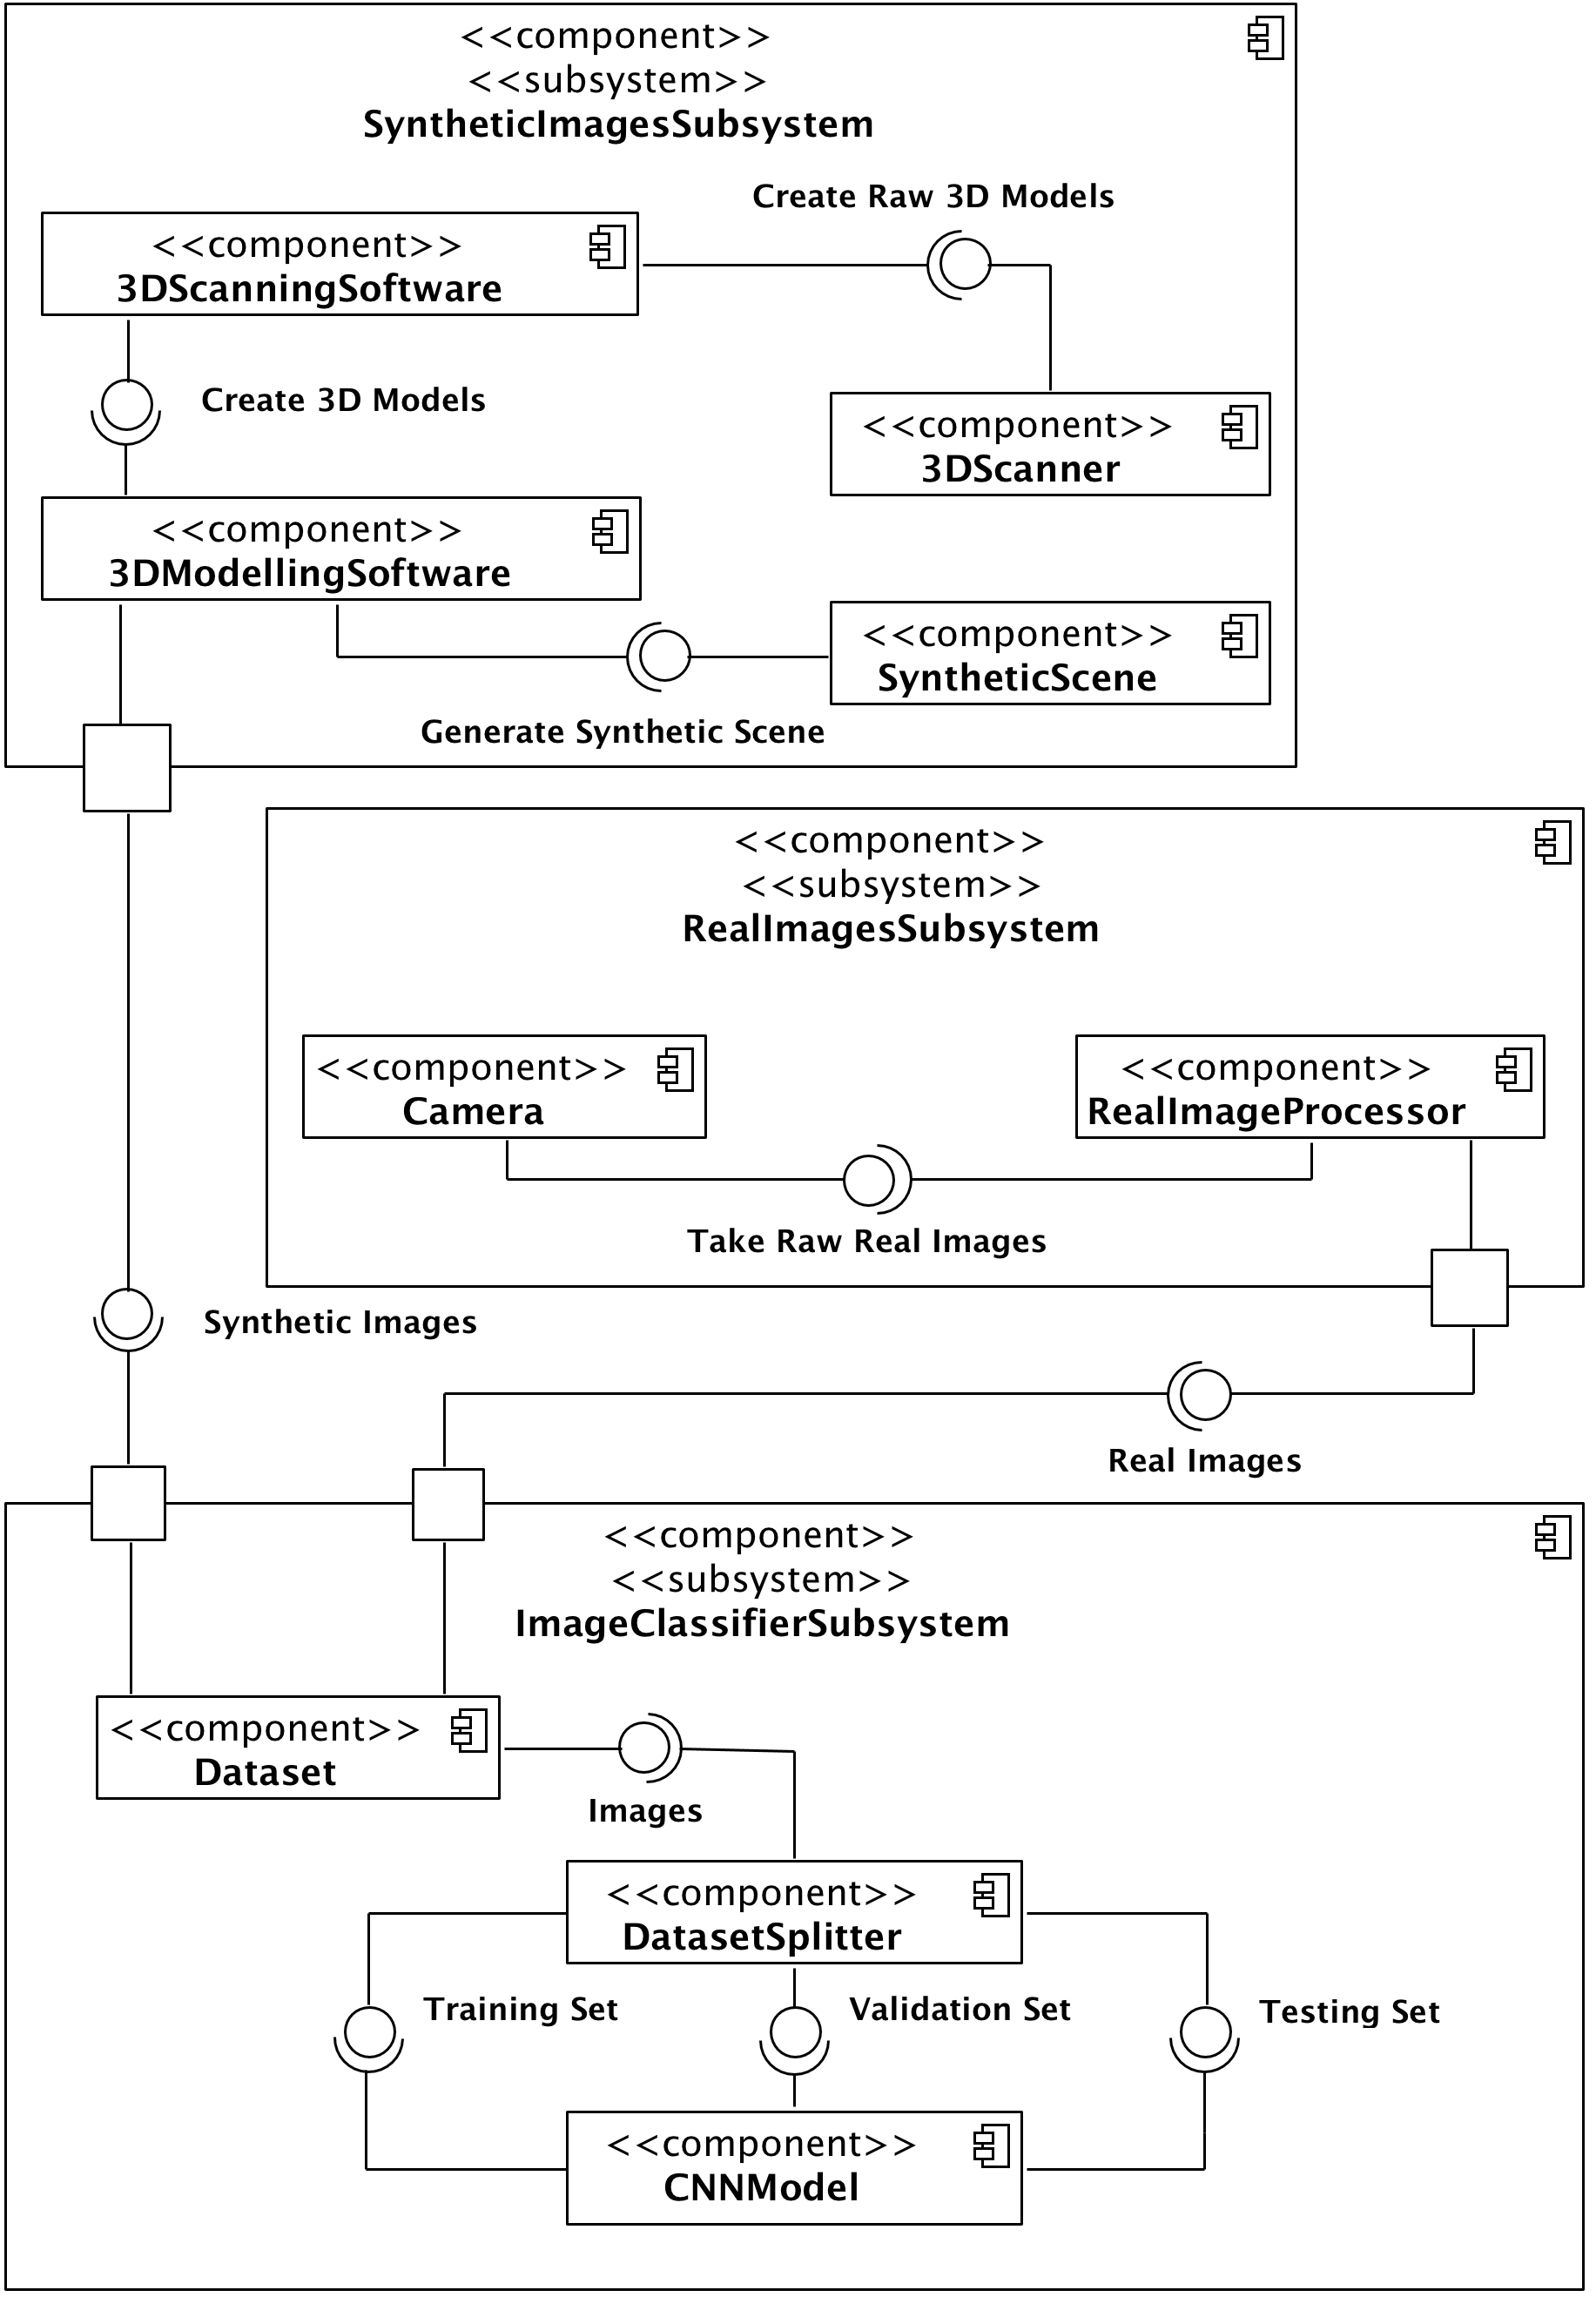
\includegraphics[width=\textwidth]{SSD}
\caption{Subsystem decomposition showing the SyntheticImageSubsystem, the RealImageSubsystem, the ImageClassifierSubsystem and the services that they provide and consume.}
\label{fig:SSD}
\end{figure}


\section{Hardware Software Mapping}\label{sec:hardware_software_mapping}

This section describes how the subsystems are mapped onto existing hardware and software components. Figure \ref{fig:DD} depicts the deployment diagram of our system. The \textbf{SyntheticImageGenerator} device is used to run 2 execution environments: the \textbf{Artec Studio}\footnote{https://www.artec3d.com/3d-software/artec-studio} 3D scanning software, and the \textbf{Rhinoceros}\footnote{https://www.rhino3d.com} 3D modeling software. Artec Studio is used to process the scans produced by the \textbf{3DScanner}\footnote{https://www.artec3d.com/portable-3d-scanners/artec-spider} device. The 3DScanner is the Artec Space Spider. The Windows version of Rhinoceros is chosen because it supports extra features that are not available on the Ubuntu or Mac versions. We use Rhinoceros to construct the SyntheticScene. Moreover, Rhinoceros hosts a \textbf{Python} execution environment. We use the Python interpreter to render synthetic images on Rhinoceros.

The \textbf{Camera} is used to capture raw images of the small parts. We use the Camera application on an iPhone 6. The \textbf{RealImageGenerator} runs a Python environment. We use the Python commands to resize the the raw images of the small parts captured by the camera. The resized real images are then ready to be fed to the image classifier.

The Dataset is stored in the file system of the \textbf{ImageClassifier} device. We use the device's Python environment to run the DatasetSplitter, the ImageClassifier, the CNNModel and the Optimizer. Furthermore, we use \textbf{Keras} \cite{chollet2015keras}, a neural networks API that provides out-of-the-box CNN implementations. The ImageClassifier device is equipped with a graphics processing unit (GPU). The GPU is used for parallel processing of the Convolutional Neural Network training algorithm. This enhancement significantly slashes down the time needed to train a CNN.

\begin{figure}[H]
\centering
  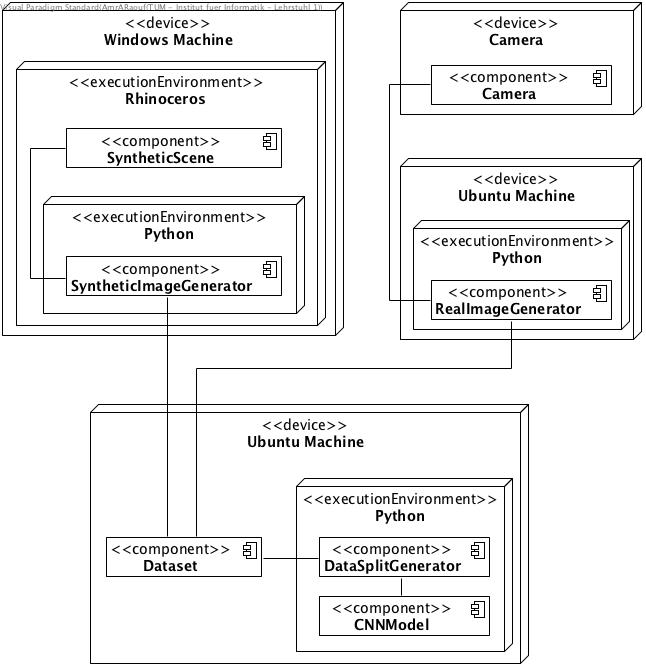
\includegraphics[width=\textwidth]{DD}
\caption{System Deployment Diagram depicting the different hardware and software components used to implement our system.}
\label{fig:DD}
\end{figure}

\section{Persistent Data Management}\label{sec:persistent_data_management}

The implementation of the ImageClassifier requires the split dataset to be organized in a certain way. The file structure of the dataset is shown in figure \ref{fig:FS}. The root folder contains 3 folders: one for training images, one for validation and one for testing. Each folder, in turn, contains one folder per class, and each of these folders are named after their respective class's label. Lastly, each class folder contains a set its own images.

\begin{figure}[H]
\centering
  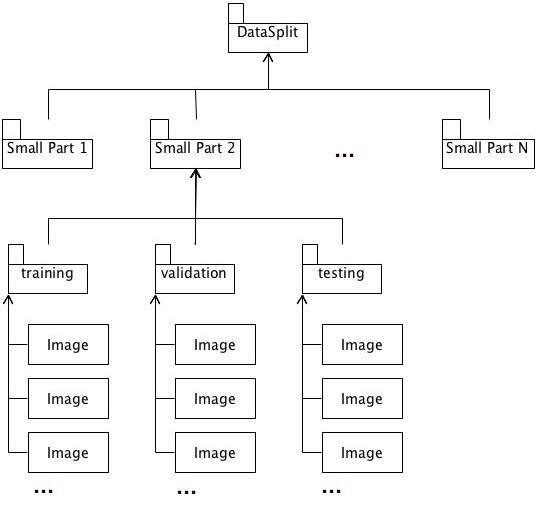
\includegraphics[width=0.8\textwidth]{FS}
\caption{Dataset file structure model displaying how the split dataset is organized before being fed as input to the image classifier. Each subfolder in the training/validation/testing directory is named after a small part label.}
\label{fig:FS}
\end{figure}
